\documentclass[11pt,a4paper]{article}
\usepackage[utf8]{inputenc}
\usepackage[T1]{fontenc}
\usepackage{lmodern}
\usepackage[english]{babel}
\usepackage[margin=2.3cm]{geometry}
\usepackage{array,booktabs,microtype,xcolor,enumitem,caption}
\usepackage[hidelinks]{hyperref}
\usepackage{pgfplots}
\pgfplotsset{compat=1.18}
\captionsetup{font=small,labelfont=bf}
\setlist{itemsep=2pt,topsep=4pt}
% Generated by paper/build.mjs from public/data/results.json (2026-11-24T15:25:46.820Z). Do not edit.

\newcommand{\NRuns}{282}
\newcommand{\NLangs}{17}
\newcommand{\TotalCost}{74.72}
\newcommand{\NFailedRoundThree}{3}
\newcommand{\NFixed}{3}
\newcommand{\CostC}{1.31}
\newcommand{\OutC}{33\,266}
\newcommand{\CodeC}{22\,502}
\newcommand{\FirstC}{100}
\newcommand{\StdC}{0}
\newcommand{\ErrC}{0}
\newcommand{\MinC}{6.1}
\newcommand{\KvDiskC}{0.0}
\newcommand{\KvBuildC}{0.1}
\newcommand{\StdBuildC}{0.1}
\newcommand{\KvProjC}{0.0}
\newcommand{\KvWtC}{0.1}
\newcommand{\StdDiskC}{0.0}
\newcommand{\SpeedC}{1.32}
\newcommand{\CostCpp}{0.97}
\newcommand{\OutCpp}{21\,789}
\newcommand{\CodeCpp}{13\,469}
\newcommand{\FirstCpp}{100}
\newcommand{\StdCpp}{0}
\newcommand{\ErrCpp}{0}
\newcommand{\MinCpp}{5.9}
\newcommand{\KvDiskCpp}{0.8}
\newcommand{\KvBuildCpp}{1.1}
\newcommand{\StdBuildCpp}{0.4}
\newcommand{\KvProjCpp}{0.8}
\newcommand{\KvWtCpp}{3.2}
\newcommand{\StdDiskCpp}{0.0}
\newcommand{\SpeedCpp}{4.31}
\newcommand{\CostRust}{0.83}
\newcommand{\OutRust}{17\,277}
\newcommand{\CodeRust}{11\,721}
\newcommand{\FirstRust}{100}
\newcommand{\StdRust}{2}
\newcommand{\ErrRust}{0}
\newcommand{\MinRust}{5.1}
\newcommand{\KvDiskRust}{107}
\newcommand{\KvBuildRust}{11.4}
\newcommand{\StdBuildRust}{1.8}
\newcommand{\KvProjRust}{76}
\newcommand{\KvWtRust}{334}
\newcommand{\StdDiskRust}{1.3}
\newcommand{\SpeedRust}{2.44}
\newcommand{\CostGo}{0.85}
\newcommand{\OutGo}{18\,221}
\newcommand{\CodeGo}{12\,141}
\newcommand{\FirstGo}{100}
\newcommand{\StdGo}{0}
\newcommand{\ErrGo}{0}
\newcommand{\MinGo}{3.1}
\newcommand{\KvDiskGo}{115}
\newcommand{\KvBuildGo}{3.1}
\newcommand{\StdBuildGo}{1.5}
\newcommand{\KvProjGo}{5.6}
\newcommand{\KvWtGo}{132}
\newcommand{\StdDiskGo}{44}
\newcommand{\SpeedGo}{1.60}
\newcommand{\CostNim}{0.85}
\newcommand{\OutNim}{15\,954}
\newcommand{\CodeNim}{7\,378}
\newcommand{\FirstNim}{75}
\newcommand{\StdNim}{2}
\newcommand{\ErrNim}{0}
\newcommand{\MinNim}{5.6}
\newcommand{\KvDiskNim}{2.7}
\newcommand{\KvBuildNim}{1.2}
\newcommand{\StdBuildNim}{0.5}
\newcommand{\KvProjNim}{2.7}
\newcommand{\KvWtNim}{11}
\newcommand{\StdDiskNim}{0.6}
\newcommand{\SpeedNim}{2.79}
\newcommand{\CostZig}{1.96}
\newcommand{\OutZig}{39\,457}
\newcommand{\CodeZig}{16\,568}
\newcommand{\FirstZig}{100}
\newcommand{\StdZig}{21}
\newcommand{\ErrZig}{3}
\newcommand{\MinZig}{9.7}
\newcommand{\KvDiskZig}{67}
\newcommand{\KvBuildZig}{9.4}
\newcommand{\StdBuildZig}{5.4}
\newcommand{\KvProjZig}{22}
\newcommand{\KvWtZig}{133}
\newcommand{\StdDiskZig}{49}
\newcommand{\SpeedZig}{1.25}
\newcommand{\CostSwift}{1.58}
\newcommand{\OutSwift}{36\,578}
\newcommand{\CodeSwift}{15\,070}
\newcommand{\FirstSwift}{8}
\newcommand{\StdSwift}{4}
\newcommand{\ErrSwift}{6}
\newcommand{\MinSwift}{11.3}
\newcommand{\KvDiskSwift}{0.1}
\newcommand{\KvBuildSwift}{9.9}
\newcommand{\StdBuildSwift}{13.8}
\newcommand{\KvProjSwift}{0.1}
\newcommand{\KvWtSwift}{0.5}
\newcommand{\StdDiskSwift}{0.1}
\newcommand{\SpeedSwift}{4.11}
\newcommand{\CostJava}{0.88}
\newcommand{\OutJava}{18\,242}
\newcommand{\CodeJava}{10\,378}
\newcommand{\FirstJava}{83}
\newcommand{\StdJava}{0}
\newcommand{\ErrJava}{0}
\newcommand{\MinJava}{5.6}
\newcommand{\KvDiskJava}{0.0}
\newcommand{\KvBuildJava}{0.4}
\newcommand{\StdBuildJava}{0.3}
\newcommand{\KvProjJava}{0.0}
\newcommand{\KvWtJava}{0.1}
\newcommand{\StdDiskJava}{0.0}
\newcommand{\SpeedJava}{3.54}
\newcommand{\CostKotlin}{0.75}
\newcommand{\OutKotlin}{14\,080}
\newcommand{\CodeKotlin}{6\,795}
\newcommand{\FirstKotlin}{100}
\newcommand{\StdKotlin}{0}
\newcommand{\ErrKotlin}{0}
\newcommand{\MinKotlin}{5.6}
\newcommand{\KvDiskKotlin}{5.8}
\newcommand{\KvBuildKotlin}{4.3}
\newcommand{\StdBuildKotlin}{2.5}
\newcommand{\KvProjKotlin}{5.8}
\newcommand{\KvWtKotlin}{23}
\newcommand{\StdDiskKotlin}{5.8}
\newcommand{\SpeedKotlin}{3.99}
\newcommand{\CostCsharp}{1.28}
\newcommand{\OutCsharp}{28\,325}
\newcommand{\CodeCsharp}{12\,075}
\newcommand{\FirstCsharp}{8}
\newcommand{\StdCsharp}{1}
\newcommand{\ErrCsharp}{2}
\newcommand{\MinCsharp}{7.7}
\newcommand{\KvDiskCsharp}{277}
\newcommand{\KvBuildCsharp}{9.5}
\newcommand{\StdBuildCsharp}{13.1}
\newcommand{\KvProjCsharp}{223}
\newcommand{\KvWtCsharp}{937}
\newcommand{\StdDiskCsharp}{195}
\newcommand{\SpeedCsharp}{3.72}
\newcommand{\CostOdin}{1.21}
\newcommand{\OutOdin}{24\,656}
\newcommand{\CodeOdin}{11\,040}
\newcommand{\FirstOdin}{50}
\newcommand{\StdOdin}{0}
\newcommand{\ErrOdin}{2}
\newcommand{\MinOdin}{6.0}
\newcommand{\KvDiskOdin}{0.3}
\newcommand{\KvBuildOdin}{1.7}
\newcommand{\StdBuildOdin}{0.5}
\newcommand{\KvProjOdin}{0.3}
\newcommand{\KvWtOdin}{1.3}
\newcommand{\StdDiskOdin}{0.1}
\newcommand{\SpeedOdin}{1.39}
\newcommand{\CostOcaml}{0.91}
\newcommand{\OutOcaml}{19\,637}
\newcommand{\CodeOcaml}{10\,227}
\newcommand{\FirstOcaml}{92}
\newcommand{\StdOcaml}{1}
\newcommand{\ErrOcaml}{0}
\newcommand{\MinOcaml}{3.9}
\newcommand{\KvDiskOcaml}{3.5}
\newcommand{\KvBuildOcaml}{0.3}
\newcommand{\StdBuildOcaml}{0.2}
\newcommand{\KvProjOcaml}{3.5}
\newcommand{\KvWtOcaml}{14}
\newcommand{\StdDiskOcaml}{1.4}
\newcommand{\SpeedOcaml}{3.06}
\newcommand{\CostHaskell}{1.10}
\newcommand{\OutHaskell}{23\,785}
\newcommand{\CodeHaskell}{9\,758}
\newcommand{\FirstHaskell}{75}
\newcommand{\StdHaskell}{2}
\newcommand{\ErrHaskell}{1}
\newcommand{\MinHaskell}{7.2}
\newcommand{\KvDiskHaskell}{1467}
\newcommand{\KvBuildHaskell}{145.6}
\newcommand{\StdBuildHaskell}{0.4}
\newcommand{\KvProjHaskell}{103}
\newcommand{\KvWtHaskell}{1775}
\newcommand{\StdDiskHaskell}{20}
\newcommand{\SpeedHaskell}{4.51}
\newcommand{\CostJs}{0.73}
\newcommand{\OutJs}{14\,259}
\newcommand{\CodeJs}{6\,522}
\newcommand{\FirstJs}{100}
\newcommand{\StdJs}{0}
\newcommand{\ErrJs}{0}
\newcommand{\MinJs}{2.9}
\newcommand{\KvDiskJs}{0.0}
\newcommand{\KvBuildJs}{0.0}
\newcommand{\StdBuildJs}{0.0}
\newcommand{\KvProjJs}{0.0}
\newcommand{\KvWtJs}{0.0}
\newcommand{\StdDiskJs}{0.0}
\newcommand{\SpeedJs}{5.65}
\newcommand{\CostTs}{0.72}
\newcommand{\OutTs}{14\,127}
\newcommand{\CodeTs}{8\,437}
\newcommand{\FirstTs}{100}
\newcommand{\StdTs}{0}
\newcommand{\ErrTs}{0}
\newcommand{\MinTs}{2.7}
\newcommand{\KvDiskTs}{0.0}
\newcommand{\KvBuildTs}{0.0}
\newcommand{\StdBuildTs}{0.0}
\newcommand{\KvProjTs}{0.0}
\newcommand{\KvWtTs}{0.0}
\newcommand{\StdDiskTs}{0.0}
\newcommand{\SpeedTs}{6.14}
\newcommand{\CostPython}{0.69}
\newcommand{\OutPython}{12\,719}
\newcommand{\CodePython}{6\,632}
\newcommand{\FirstPython}{92}
\newcommand{\StdPython}{0}
\newcommand{\ErrPython}{0}
\newcommand{\MinPython}{2.8}
\newcommand{\KvDiskPython}{0.0}
\newcommand{\KvBuildPython}{0.0}
\newcommand{\StdBuildPython}{0.0}
\newcommand{\KvProjPython}{0.0}
\newcommand{\KvWtPython}{0.1}
\newcommand{\StdDiskPython}{0.0}
\newcommand{\SpeedPython}{6.52}
\newcommand{\CostAsm}{3.28}
\newcommand{\OutAsm}{99\,286}
\newcommand{\CodeAsm}{36\,769}
\newcommand{\FirstAsm}{58}
\newcommand{\StdAsm}{0}
\newcommand{\ErrAsm}{1}
\newcommand{\MinAsm}{15.8}
\newcommand{\KvDiskAsm}{0.0}
\newcommand{\KvBuildAsm}{0.1}
\newcommand{\StdBuildAsm}{0.1}
\newcommand{\KvProjAsm}{0.0}
\newcommand{\KvWtAsm}{0.1}
\newcommand{\StdDiskAsm}{0.0}
\newcommand{\SpeedAsm}{1.06}
\newcommand{\CorrCodeCost}{0.92}
\newcommand{\CorrCodeCostSpearman}{0.85}
\newcommand{\CorrCostSpeed}{0.63}
\newcommand{\FastestLang}{Assembly}
\newcommand{\KvPointsMin}{53}
\newcommand{\CorrCodeCostNoAsm}{0.71}
\newcommand{\TsJsCode}{1.29}
\newcommand{\TsJsCodeClk}{1.26}
\newcommand{\TsJsCost}{0.98}
\newcommand{\NTrackRuns}{60}
\newcommand{\NTrackLangs}{10}
\newcommand{\NTrackFailed}{0}
\newcommand{\NTrackFixed}{0}
\newcommand{\TrkNumericOctave}{0.48}
\newcommand{\TrkNumericJulia}{0.46}
\newcommand{\TrkNumericR}{0.31}
\newcommand{\TrkProofsLean}{0.28}
\newcommand{\TrkProofsRocq}{0.28}
\newcommand{\TrkProofsDafny}{0.25}
\newcommand{\TrkEvmSolidity}{0.42}
\newcommand{\TrkEvmVyper}{0.41}
\newcommand{\TrkZkCircom}{0.46}
\newcommand{\TrkZkNoir}{0.47}
\newcommand{\NSkillLangs}{0}
\newcommand{\NSkillCheaper}{0}
\newcommand{\NSkillWorksUp}{0}
\newcommand{\NSkillWorksDown}{0}
\newcommand{\SkillMedianChange}{--}
\newcommand{\SkillAuthorCost}{0.00}
\newcommand{\CorrStdCost}{0.32}
\newcommand{\DevloopRust}{206}
\newcommand{\DevloopRustWt}{857}
\newcommand{\NDepsLangs}{2}
\newcommand{\CheapestLang}{Python}
\newcommand{\CostCheapest}{0.69}
\newcommand{\ShortestLang}{JavaScript}
\newcommand{\RatioC}{1.9}
\newcommand{\RatioCpp}{1.4}
\newcommand{\RatioRust}{1.2}
\newcommand{\RatioGo}{1.2}
\newcommand{\RatioNim}{1.2}
\newcommand{\RatioZig}{2.9}
\newcommand{\RatioSwift}{2.3}
\newcommand{\RatioJava}{1.3}
\newcommand{\RatioKotlin}{1.1}
\newcommand{\RatioCsharp}{1.9}
\newcommand{\RatioOdin}{1.8}
\newcommand{\RatioOcaml}{1.3}
\newcommand{\RatioHaskell}{1.6}
\newcommand{\RatioJs}{1.1}
\newcommand{\RatioTs}{1.1}
\newcommand{\RatioPython}{1.0}
\newcommand{\RatioAsm}{4.8}
\newcommand{\ComboJsSvelte}{2\,736}
\newcommand{\ComboKotlinSvelte}{2\,775}
\newcommand{\ComboJsVue}{2\,790}
\newcommand{\ComboKotlinVue}{2\,829}
\newcommand{\ComboJsReact}{2\,994}
\newcommand{\ComboKotlinReact}{3\,033}
\newcommand{\ComboTsSvelte}{3\,219}
\newcommand{\ComboTsVue}{3\,273}
\newcommand{\ComboHaskellSvelte}{3\,308}
\newcommand{\ComboHaskellVue}{3\,362}
\newcommand{\ComboJavaSvelte}{3\,460}
\newcommand{\ComboTsReact}{3\,477}
\newcommand{\ComboJavaVue}{3\,514}
\newcommand{\ComboHaskellReact}{3\,566}
\newcommand{\ComboRustSvelte}{3\,702}
\newcommand{\ComboJavaReact}{3\,718}
\newcommand{\ComboRustVue}{3\,756}
\newcommand{\ComboRustReact}{3\,960}
\newcommand{\ComboNimSvelte}{4\,056}
\newcommand{\ComboNimVue}{4\,110}
\newcommand{\ComboPythonSvelte}{4\,148}
\newcommand{\ComboPythonVue}{4\,202}
\newcommand{\ComboNimReact}{4\,314}
\newcommand{\ComboPythonReact}{4\,406}
\newcommand{\ComboCsharpSvelte}{4\,432}
\newcommand{\ComboCsharpVue}{4\,486}
\newcommand{\ComboCsharpReact}{4\,690}
\newcommand{\ComboGoSvelte}{5\,442}
\newcommand{\ComboGoVue}{5\,496}
\newcommand{\ComboGoReact}{5\,700}
\newcommand{\ComboOdinSvelte}{5\,810}
\newcommand{\ComboOdinVue}{5\,864}
\newcommand{\ComboOcamlSvelte}{6\,006}
\newcommand{\ComboOcamlVue}{6\,060}
\newcommand{\ComboOdinReact}{6\,068}
\newcommand{\ComboOcamlReact}{6\,264}
\newcommand{\ComboSwiftSvelte}{8\,017}
\newcommand{\ComboSwiftVue}{8\,071}
\newcommand{\ComboSwiftReact}{8\,275}
\newcommand{\ComboZigSvelte}{8\,565}
\newcommand{\ComboZigVue}{8\,619}
\newcommand{\ComboCppSvelte}{8\,637}
\newcommand{\ComboCppVue}{8\,691}
\newcommand{\ComboZigReact}{8\,823}
\newcommand{\ComboCppReact}{8\,895}
\newcommand{\ComboCSvelte}{12\,743}
\newcommand{\ComboCVue}{12\,797}
\newcommand{\ComboCReact}{13\,001}
\newcommand{\ComboAsmSvelte}{16\,803}
\newcommand{\ComboAsmVue}{16\,857}
\newcommand{\ComboAsmReact}{17\,061}

\newcommand{\LeaderboardTable}{%
\begin{tabular}{@{}lrrrrrrrrr@{}}
\toprule
Language & Solved & 1st try & US\$ & Output & Turns & Min & Code & Errors & Stdlib \\
\midrule
Python & 12/12 & 92\% & 0.69 & 12\,719 & 17 & 2.8 & 6\,632 & 0.0 & 0 \\
TypeScript & 12/12 & 100\% & 0.72 & 14\,127 & 16 & 2.7 & 8\,437 & 0.0 & 0 \\
JavaScript & 12/12 & 100\% & 0.73 & 14\,259 & 17 & 2.9 & 6\,522 & 0.0 & 0 \\
Kotlin & 12/12 & 100\% & 0.75 & 14\,080 & 20 & 5.6 & 6\,795 & 0.0 & 0 \\
Rust & 12/12 & 100\% & 0.83 & 17\,277 & 18 & 5.1 & 11\,721 & 0.0 & 2 \\
Nim & 12/12 & 75\% & 0.85 & 15\,954 & 23 & 5.6 & 7\,378 & 0.0 & 2 \\
Go & 12/12 & 100\% & 0.85 & 18\,221 & 17 & 3.1 & 12\,141 & 0.0 & 0 \\
Java & 12/12 & 83\% & 0.88 & 18\,242 & 22 & 5.6 & 10\,378 & 0.0 & 0 \\
OCaml & 12/12 & 92\% & 0.91 & 19\,637 & 25 & 3.9 & 10\,227 & 0.0 & 1 \\
C++ & 12/12 & 100\% & 0.97 & 21\,789 & 20 & 5.9 & 13\,469 & 0.0 & 0 \\
Haskell & 12/12 & 75\% & 1.10 & 23\,785 & 33 & 7.2 & 9\,758 & 1.0 & 2 \\
Odin & 9/12 & 50\% & 1.21 & 24\,656 & 37 & 6.0 & 11\,040 & 2.0 & 0 \\
C\# & 12/12 & 8\% & 1.28 & 28\,325 & 36 & 7.7 & 12\,075 & 2.0 & 1 \\
C & 12/12 & 100\% & 1.31 & 33\,266 & 25 & 6.1 & 22\,502 & 0.0 & 0 \\
Swift & 12/12 & 8\% & 1.58 & 36\,578 & 39 & 11.3 & 15\,070 & 6.0 & 4 \\
Zig & 12/12 & 100\% & 1.96 & 39\,457 & 48 & 9.7 & 16\,568 & 3.0 & 21 \\
Assembly & 12/12 & 58\% & 3.28 & 99\,286 & 37 & 15.8 & 36\,769 & 1.0 & 0 \\
\bottomrule
\end{tabular}}

\newcommand{\CostPlot}{%
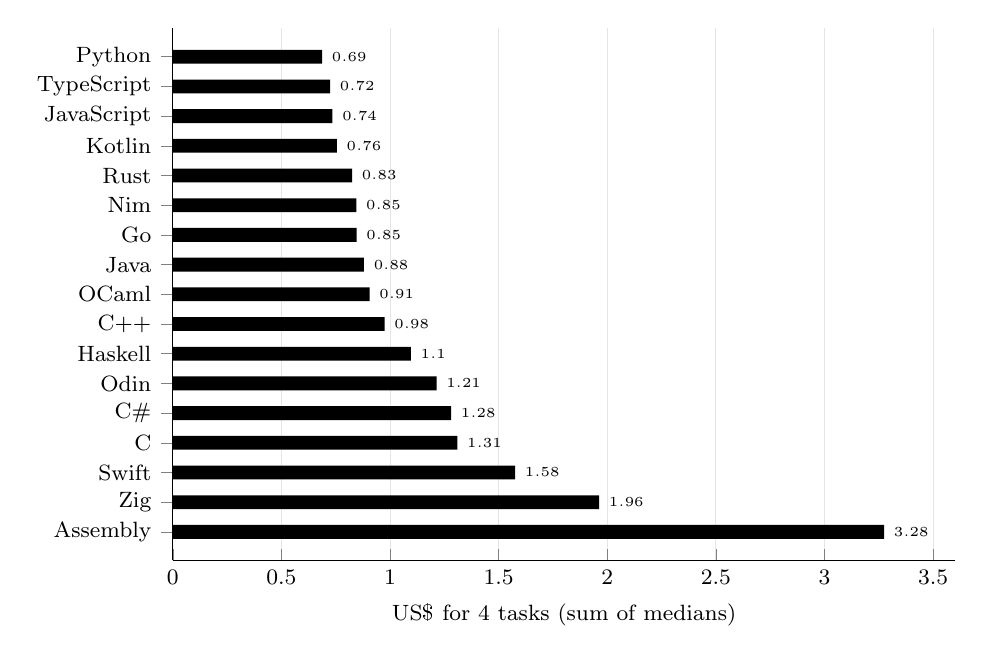
\begin{tikzpicture}
\begin{axis}[xbar, width=0.95\columnwidth, height=8.34cm, bar width=5pt, xmin=0,
  symbolic y coords={Asm,Zig,Swift,C,Csharp,Odin,Haskell,Cpp,Ocaml,Java,Go,Nim,Rust,Kotlin,Js,Ts,Python}, ytick=data, yticklabels={Assembly,Zig,Swift,C,C\#,Odin,Haskell,C++,OCaml,Java,Go,Nim,Rust,Kotlin,JavaScript,TypeScript,Python},
  xlabel={US\$ for 4 tasks (sum of medians)}, nodes near coords, nodes near coords style={font=\tiny}, every node near coord/.append style={/pgf/number format/.cd, fixed, precision=2, use period},
  tick label style={font=\footnotesize}, label style={font=\footnotesize}, axis x line*=bottom, axis y line*=left, enlarge y limits=0.06, xmajorgrids, major grid style={gray!20}]
\addplot[fill=black, draw=none] coordinates {(3.275,Asm) (1.963,Zig) (1.576,Swift) (1.310,C) (1.281,Csharp) (1.214,Odin) (1.096,Haskell) (0.975,Cpp) (0.906,Ocaml) (0.880,Java) (0.846,Go) (0.845,Nim) (0.825,Rust) (0.755,Kotlin) (0.735,Js) (0.724,Ts) (0.687,Python)};
\end{axis}
\end{tikzpicture}}

\newcommand{\CodePlot}{%
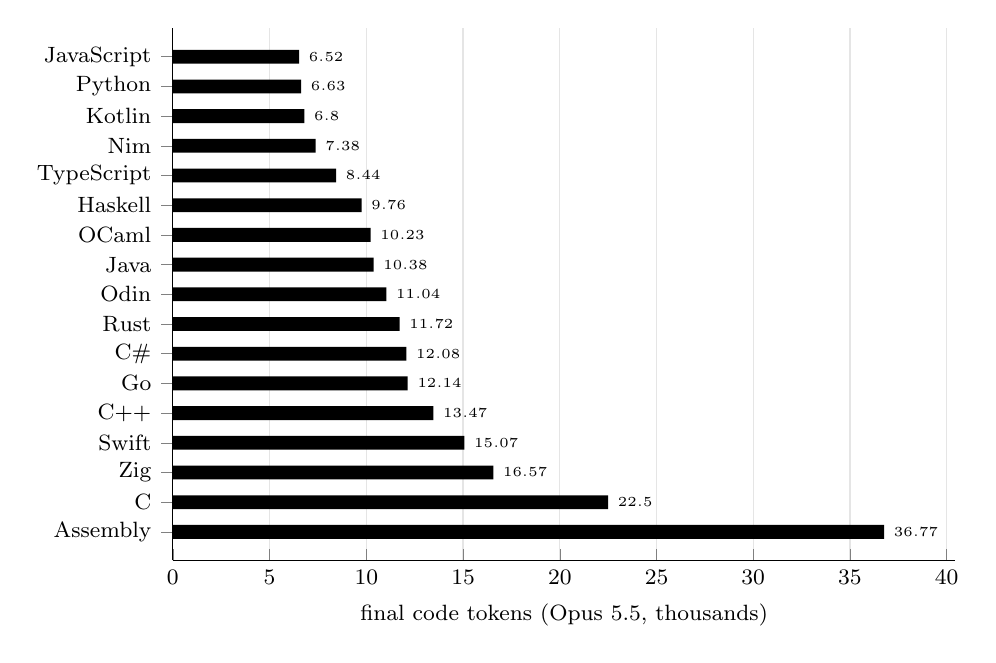
\begin{tikzpicture}
\begin{axis}[xbar, width=0.95\columnwidth, height=8.34cm, bar width=5pt, xmin=0,
  symbolic y coords={Asm,C,Zig,Swift,Cpp,Go,Csharp,Rust,Odin,Java,Ocaml,Haskell,Ts,Nim,Kotlin,Python,Js}, ytick=data, yticklabels={Assembly,C,Zig,Swift,C++,Go,C\#,Rust,Odin,Java,OCaml,Haskell,TypeScript,Nim,Kotlin,Python,JavaScript},
  xlabel={final code tokens (Opus 5.5, thousands)}, nodes near coords, nodes near coords style={font=\tiny}, every node near coord/.append style={/pgf/number format/.cd, fixed, precision=2, use period},
  tick label style={font=\footnotesize}, label style={font=\footnotesize}, axis x line*=bottom, axis y line*=left, enlarge y limits=0.06, xmajorgrids, major grid style={gray!20}]
\addplot[fill=black, draw=none] coordinates {(36.769,Asm) (22.502,C) (16.568,Zig) (15.070,Swift) (13.469,Cpp) (12.141,Go) (12.075,Csharp) (11.721,Rust) (11.040,Odin) (10.378,Java) (10.227,Ocaml) (9.758,Haskell) (8.437,Ts) (7.378,Nim) (6.795,Kotlin) (6.632,Python) (6.522,Js)};
\end{axis}
\end{tikzpicture}}

\newcommand{\KvTable}{%
\begin{tabular}{@{}l>{\raggedright\arraybackslash}p{3.6cm}rrr@{}}
\toprule
Language & Dependencies (most common) & MB & Build s & req/s \\
\midrule
Haskell & bytestring, containers, http-types, wai, warp & 1467 & 145.6 & 23\,610 \\
C\# & stdlib & 277 & 9.5 & 22\,434 \\
Go & stdlib & 115 & 3.1 & 24\,521 \\
Rust & bytes, http-body-util, hyper, hyper-util, tokio & 107 & 11.4 & 17\,513 \\
Zig & stdlib & 67 & 9.4 & 26\,144 \\
Kotlin & stdlib & 5.8 & 4.3 & 21\,422 \\
OCaml & stdlib & 3.5 & 0.3 & 24\,709 \\
Nim & stdlib & 2.7 & 1.2 & 22\,069 \\
C++ & stdlib & 0.8 & 1.1 & 24\,017 \\
Odin & stdlib & 0.3 & 1.7 & 23\,677 \\
Swift & stdlib & 0.1 & 9.9 & 14\,837 \\
C & stdlib & 0.0 & 0.1 & 27\,776 \\
Java & stdlib & 0.0 & 0.4 & 22\,763 \\
Assembly & stdlib & 0.0 & 0.1 & 22\,051 \\
Python & stdlib & 0.0 & 0.0 & 27\,272 \\
JavaScript & stdlib & 0.0 & 0.0 & 24\,608 \\
TypeScript & stdlib & 0.0 & 0.0 & 25\,275 \\
\bottomrule
\end{tabular}}

\newcommand{\PerfTable}{%
\begin{tabular}{@{}lrrrr@{}}
\toprule
Language & wordfreq ms & lru ms & calc ms & lru RSS MB \\
\midrule
Assembly & 94 & 36 & 18 & 29 \\
Zig & 119 & 56 & 21 & 28 \\
Odin & 158 & 59 & 21 & 39 \\
C & 135 & 52 & 26 & 30 \\
Go & 169 & 80 & 26 & 20 \\
Rust & 244 & 180 & 31 & 42 \\
Nim & 308 & 245 & 39 & 58 \\
OCaml & 366 & 241 & 54 & 18 \\
Haskell & 1\,100 & 218 & 89 & 117 \\
Swift & 194 & 525 & 91 & 8.5 \\
C\# & 315 & 330 & 91 & 113 \\
Java & 182 & 290 & 149 & 138 \\
Kotlin & 230 & 349 & 149 & 152 \\
JavaScript & 837 & 350 & 188 & 262 \\
TypeScript & 861 & 365 & 251 & 285 \\
C++ & 200 & 223 & 406 & 43 \\
Python & 607 & 346 & 516 & 184 \\
\bottomrule
\end{tabular}}

\newcommand{\SpeedTable}{%
\begin{tabular}{@{}rlrrrrrr@{}}
\toprule
\# & Language & wordfreq & lru & calc & kvhttp & Score & $\times$fastest \\
\midrule
1 & Assembly & 100 & 100 & 100 & 79 & \textbf{94.4} & 1.06 \\
2 & Zig & 79 & 64 & 86 & 94 & \textbf{80.0} & 1.25 \\
3 & C & 70 & 69 & 69 & 100 & \textbf{76.0} & 1.32 \\
4 & Odin & 59 & 61 & 86 & 85 & \textbf{71.8} & 1.39 \\
5 & Go & 56 & 45 & 69 & 88 & \textbf{62.5} & 1.60 \\
6 & Rust & 39 & 20 & 58 & 63 & \textbf{41.0} & 2.44 \\
7 & Nim & 31 & 15 & 46 & 79 & \textbf{35.8} & 2.79 \\
8 & OCaml & 26 & 15 & 33 & 89 & \textbf{32.7} & 3.06 \\
9 & Java & 52 & 12 & 12 & 82 & \textbf{28.2} & 3.54 \\
10 & C\# & 30 & 11 & 20 & 81 & \textbf{26.9} & 3.72 \\
11 & Kotlin & 41 & 10 & 12 & 77 & \textbf{25.0} & 3.99 \\
12 & Swift & 48 & 7 & 20 & 53 & \textbf{24.3} & 4.11 \\
13 & C++ & 47 & 16 & 4 & 86 & \textbf{23.2} & 4.31 \\
14 & Haskell & 9 & 17 & 20 & 85 & \textbf{22.2} & 4.51 \\
15 & JavaScript & 11 & 10 & 10 & 89 & \textbf{17.7} & 5.65 \\
16 & TypeScript & 11 & 10 & 7 & 91 & \textbf{16.3} & 6.14 \\
17 & Python & 15 & 10 & 3 & 98 & \textbf{15.3} & 6.52 \\
\bottomrule
\end{tabular}}

\newcommand{\FrontTable}{%
\begin{tabular}{@{}lrrrrr>{\raggedright\arraybackslash}p{3cm}@{}}
\toprule
 & Article & Ours & Ours & ui & shop & Store in shop \\
 & cl100k & cl100k & Opus & tokens & tokens & (agent's choice) \\
\midrule
React & 1.254 & 1.217 & 1.264 & 2\,599 & 3\,348 & Context + useReducer \\
Svelte & 1.000 & 1.000 & 1.000 & 2\,056 & 2\,543 & Svelte runes (\$state) \\
Vue & 1.115 & 1.090 & 1.108 & 2\,278 & 2\,581 & Vue reactive(), Pinia \\
\bottomrule
\end{tabular}}

\newcommand{\TrackTable}{%
\begin{tabular}{@{}llrrrrrrr@{}}
\toprule
Track & Language & Solved & Repaired & 1st try & US\$ & Output & Code & Turns \\
\midrule
Scientific computing & R & 6/6 & 6/6 & 100\% & 0.31 & 4\,329 & 2\,135 & 10 \\
 & Julia & 6/6 & 6/6 & 83\% & 0.46 & 9\,867 & 5\,386 & 10 \\
 & Octave & 6/6 & 6/6 & 100\% & 0.48 & 8\,596 & 1\,923 & 20 \\
\midrule
Theorem proving & Dafny & 6/6 & 6/6 & 100\% & 0.25 & 2\,285 & 2\,260 & 7 \\
 & Lean 4 & 6/6 & 6/6 & 83\% & 0.28 & 2\,777 & 1\,892 & 9 \\
 & Rocq & 6/6 & 6/6 & 100\% & 0.28 & 2\,944 & 2\,043 & 8 \\
\midrule
Smart contracts & Vyper & 6/6 & 6/6 & 100\% & 0.41 & 5\,757 & 3\,973 & 9 \\
 & Solidity & 6/6 & 6/6 & 100\% & 0.42 & 5\,947 & 3\,432 & 8 \\
\midrule
Zero-knowledge circuits & Circom & 6/6 & 6/6 & 83\% & 0.46 & 8\,613 & 3\,032 & 13 \\
 & Noir & 6/6 & 6/6 & 33\% & 0.47 & 7\,330 & 3\,169 & 12 \\
\bottomrule
\end{tabular}}

\newcommand{\SkillTable}{%
\begin{tabular}{@{}lrrrrrrrr@{}}
\toprule
Language & Works & US\$ & $\Delta$US\$ & $\Delta$Output & Errors & Used & Skill US\$ & Pays off \\
\midrule

\bottomrule
\end{tabular}}

\newcommand{\SkillSlope}{%

\begin{tikzpicture}
\node[anchor=east, font=\footnotesize\bfseries] at (-0.1,0.5) {Without skill};
\node[anchor=west, font=\footnotesize\bfseries] at (4.1,0.5) {With skill};

\end{tikzpicture}}


\title{\textbf{How Much Does a Programming Language Cost a Coding Agent?}\\[4pt]
\large Tokens, Time and Correctness with Claude Opus 5.5\\across \NLangs{} Languages and Three Front-End Frameworks}
\author{Arthur De Freitas Abeilice\\
\small Universidade Federal de Minas Gerais (UFMG)\\
\small\texttt{abeilice@ufmg.br} \quad \url{https://github.com/afa7789/TKNbenchmark}}
\date{November 2026}

\begin{document}
\maketitle

\begin{abstract}
\noindent
We measure how much a coding agent spends to solve the same tasks in \NLangs{} programming languages
and in React, Vue and Svelte. Every case (language $\times$ task $\times$ repetition) was run by its own
isolated Claude Opus 5.5 agent with an identical prompt, and checked live by hidden tests, a clean build
and, for front ends, a real browser. Across \NRuns{} agent runs, \NFailedRoundThree{} failed verification and
\NFixed{} of them were fixed by a repair agent that received the failure report. The language barely
changed correctness, but it changed the cost: from the cheapest (\CheapestLang, US\$\,\CostCheapest{} for
four tasks) to the most expensive (Assembly) the gap was \RatioAsm$\times$. Python, TypeScript and
JavaScript were the three cheapest. Final code size tracks cost closely (Spearman $\rho =
\CorrCodeCostSpearman$) but not completely: Zig cost \RatioZig$\times$ the cheapest, more than C, whose
code is larger, because the agent had to read the standard library's source to learn a recently changed
API. TypeScript's code was \TsJsCodeClk$\times$ JavaScript's in \texttt{cl100k} tokens, close to the
1.31$\times$ reported for snippets, yet the agent spent the same on both. Rust's build artifacts live per
project, so parallel agent worktrees multiply them. For front ends we reproduce the published ordering
(Svelte $<$ Vue $<$ React) with a different tokenizer.
\end{abstract}

\section{Motivation and hypotheses}

Pereira et al.~\cite{pereira2017} asked how energy, time and memory relate when the same programs
are written in 27 languages. Coding agents add a fourth resource to that list: the tokens spent to
produce, test and fix the program. The series \emph{The Tokenomics of Web
Development}~\cite{tokenomics1,tokenomics2} measured, with \texttt{tiktoken}, the token size of
hand-written idiomatic snippets: Angular costs 38\% more than Svelte,
TypeScript 31\% more than JavaScript. An agent, however, does more than emit code: it reads the
specification, compiles, fails, reads error messages, looks things up and tries again. We wanted to know
whether the choice of language changes that whole bill. A conversation between two developers, one of
them running Rust + React in a server for chat bots, supplied the hypotheses:

\begin{description}[leftmargin=1.2em]
  \item[H1 (Zig)] Zig spends fewer tokens than Rust, compiles faster and is simpler for an LLM to get
        right on the first try.
  \item[H2 (Rust disk)] Rust produces very large \texttt{target/} directories, which hurts when agents
        work in parallel worktrees.
  \item[H3 (conciseness)] More concise languages cost the agent fewer tokens, as the series showed for
        static snippets.
  \item[H4 (front end)] Svelte $<$ Vue $<$ React in tokens~\cite{tokenomics1}.
  \item[H5 (Rust + React)] Rust + React is a good stack for people who program with agents.
\end{description}

\section{Related work}

\paragraph{Comparing programming languages.} Empirical comparisons of languages solving the same
problems go back at least to Prechelt~\cite{prechelt2000}, who compared seven languages on one task for
program length, development effort, run time and memory. Nanz and Furia~\cite{nanz2015} compared eight
languages on Rosetta Code for conciseness, size, speed and failures. Closest in spirit to this work,
Pereira et al.~\cite{pereira2017,pereira2021} ran the Computer Language Benchmarks Game in 27 languages
and related energy, time and memory; we keep their design (the same problems across many languages, one
resource measured at a time) and measure the tokens an agent spends instead. Ray et
al.~\cite{ray2014} and the reproduction by Berger et al.~\cite{berger2019} show how hard it is to
attribute outcomes to the language alone, a caveat that applies here too.

\paragraph{Language models and code across languages.} HumanEval~\cite{humaneval} measured the
functional correctness of generated Python. MultiPL-E~\cite{multiple} translated it into 18 more
languages and found that model performance depends on how common a language is and on its features,
which matches our finding that the model's familiarity with a language version drives the cost.

\paragraph{Coding agents.} SWE-bench~\cite{swebench} evaluates models on real GitHub issues from
Python repositories; SWE-agent~\cite{sweagent} showed that the agent--computer interface changes the
outcome; DeepSWE~\cite{deepswe} reports cost and steps alongside pass@1. These benchmarks hold the
language fixed and vary the model. We hold the model and harness fixed and vary the language.

\section{Method}

\paragraph{Agents.} Inspired by DeepSWE~\cite{deepswe}, each case runs its own headless Claude Code
(\texttt{claude -p}): model \texttt{claude-opus-5-5}, effort \texttt{high}, tools \texttt{Bash},
\texttt{Read}, \texttt{Edit} and \texttt{Write}; no web, MCP, plugins or \texttt{CLAUDE.md}; an empty
directory outside the repository. The prompt is the same for every language except for the language name
and toolchain version (Assembly, the JVM languages, JavaScript, TypeScript and Python get one extra line: ``only
\texttt{.s}, libc calls allowed'', or ``\texttt{./app} may be a launcher script that runs
\texttt{java}/\texttt{node}/\texttt{python3}''). The agent sees the
specification, a few examples and the \texttt{check.mjs} script that runs them.

\paragraph{Tasks.} Four back-end programs: \texttt{wordfreq} (bytes, hash maps, sorting, inputs up to
50\,MB), \texttt{lru} (an LRU cache over one million commands), \texttt{calc} (a recursive-descent
parser with \texttt{int64} overflow rules) and \texttt{kvhttp} (a concurrent HTTP key--value server,
where third-party packages are allowed). The first three are standard-library only. For front ends,
\texttt{ui} (the series' five components plus a client for \texttt{kvhttp}) and \texttt{shop} (a mini
app with parent/child components, a global store of the agent's choice, derived state, a form, an effect
with cleanup, context and slots). Three repetitions per case.

\paragraph{Rounds.} (1--2) Write. (3) Verify once, live: for back ends, a cold build of a clean copy with
isolated caches and a hidden suite larger than the examples; for front ends, a Vite build and checks in
Chromium with mocked network, testing only what the specification states literally plus the absence of
runtime errors. (4) Repair: each failure gets a fresh agent with the failure report, up to three
attempts. Each verifier was first validated against reference implementations.

\paragraph{Metrics.} Tokens and cost come from Claude Code's final event (Opus 5.5 list price: US\$\,4
and 20 per million input and output tokens, cache included). Final code was counted with Opus 5.5's own
tokenizer, as the input-token difference between a prompt with the code and an empty one, and also with
\texttt{cl100k\_base} to compare with the series. We also count compiler errors and reads of the
toolchain's own sources or docs, binary performance (median of five runs) and server throughput with 64
concurrent clients. Disk is split into per-project artifacts and shared global caches, so that the cost
of $N$ worktrees is $N \times \mathrm{project} + \mathrm{cache}$.

\section{Results}

Table~\ref{tab:main} and Figure~\ref{fig:cost} summarise the back ends; costs are the sum of the
per-task medians over the four tasks. Of the \NRuns{} runs, \NFailedRoundThree{} failed round 3, all of
them Odin \texttt{calc} on the same hidden random case; the repair round fixed each on the first attempt.

\begin{table}[h]
\centering\small
\caption{Per language, summing the medians of the 4 tasks. ``Solved'': passed the hidden suite in
round 3. ``1st try'': the first run of the examples already passed. ``Code'': Opus 5.5 tokens of the
final code. ``Stdlib'': reads of the toolchain's own sources/docs.}
\label{tab:main}
\LeaderboardTable
\end{table}

\begin{figure}[h]
\centering
\begin{minipage}{0.49\linewidth}\centering\CostPlot\end{minipage}\hfill
\begin{minipage}{0.49\linewidth}\centering\CodePlot\end{minipage}
\caption{Agent cost (left) and final code size (right), per language.}
\label{fig:cost}
\end{figure}

\begin{table}[h]
\centering\small
\caption{\texttt{kvhttp}: dependencies chosen by the agent, disk after a cold build (project + caches it
created), build time and throughput.}
\label{tab:kv}
\KvTable
\end{table}

\begin{table}[h]
\centering\small
\caption{Final binary performance (median of 5 runs), including process start-up (and JVM start-up for
Java and Kotlin).}
\label{tab:perf}
\PerfTable
\end{table}

\begin{table}[h]
\centering\small
\caption{Front end. Ratios to Svelte (= 1): the article~\cite{tokenomics1} and our measurement.}
\label{tab:front}
\FrontTable
\end{table}

\section{Discussion}

\paragraph{H1 (Zig): rejected in this setting.} Zig cost US\$\,\CostZig{} against US\$\,\CostRust{} for
Rust. It did not fail more often (\FirstZig\% passed on the first try, as Rust did); it spent the money
learning. The agent made \StdZig{} reads of the Zig~0.16 standard library sources, whose I/O API
changed recently, against \StdRust{} for Rust. Cold builds were not faster either: \StdBuildZig\,s
against \StdBuildRust\,s on the standard-library tasks, because Zig compiles its standard library from
source into an empty cache. A simple language is not enough; the model must know the version in use.

\paragraph{H2 (Rust disk): confirmed once dependencies and worktrees enter.} Without dependencies Rust is
light: \StdDiskRust\,MB after the build, against \StdDiskZig\,MB for Zig. For the HTTP server Rust and
Haskell were the only languages whose agents pulled in packages (\texttt{tokio} and
\texttt{hyper}/\texttt{axum}; \texttt{warp}), and Rust's release build reached \KvDiskRust\,MB and \KvBuildRust\,s. What matters is where those bytes live.
\texttt{target/} is per project (\KvProjRust\,MB for the release build alone), so every worktree
repeats it, while Go keeps almost everything in its global cache (\KvProjGo\,MB per project). With four
worktrees Rust reaches \KvWtRust\,MB and Go \KvWtGo\,MB. After a full development loop (debug build,
release build and test build) Rust's \texttt{target/} reached \DevloopRust\,MB per worktree, or
\DevloopRustWt\,MB for four, for a server of about 200 lines. With hundreds of crates and incremental
builds this becomes the gigabytes that people running parallel agents report. Rust is not alone, though:
per project, the release builds of C\# (\KvProjCsharp\,MB in \texttt{bin/} and \texttt{obj/}) and
Haskell (\KvProjHaskell\,MB in \texttt{dist-newstyle/}, plus a shared cabal store; \KvDiskHaskell\,MB
in total) were larger than Rust's, giving \KvWtCsharp\,MB and \KvWtHaskell\,MB for four worktrees.

\paragraph{H3 (conciseness): confirmed for code, with caveats for cost.} Across languages, final code
size and agent cost are strongly associated: Spearman $\rho = \CorrCodeCostSpearman$, Pearson $r =
\CorrCodeCost$, or $r = \CorrCodeCostNoAsm$ without Assembly, which is an outlier on both axes. The four
cheapest languages (Python, TypeScript, JavaScript and Kotlin) include the three with the least code
(\ShortestLang, Python and Kotlin). The more verbose Java cost more than Kotlin. C cost more than C++
because, lacking hash maps and strings in its standard library, it has to write more; Assembly was the
extreme (\RatioAsm$\times$). The series' headline comparison replicates for code but not for cost:
TypeScript's final code was \TsJsCodeClk$\times$ JavaScript's in \texttt{cl100k} tokens (the series
reports 1.31$\times$ for snippets) and \TsJsCode$\times$ in Opus tokens, but the agent's cost ratio was
\TsJsCost$\times$. Type annotations add tokens to the artefact, not to the process that writes it. The
exceptions tell the other half of the story. Zig cost more than C, whose code is larger, because the agent paid for API uncertainty
(\StdZig{} standard-library reads); Odin was the only language whose agents failed hidden tests. Swift
and C\# also cost more than their code size predicts, but for a reason outside the languages: on the test
machine, which has Apple's Command Line Tools but no Xcode, SwiftPM aborts at start-up and .NET Native AOT
cannot link, so the agents' first builds failed (only \FirstSwift\% and \FirstCsharp\% passed on the
first try) until they found a workaround (calling \texttt{swiftc} directly; a non-AOT build).

\paragraph{H4 (front end): confirmed.} With a different component set, written by agents, and with
Opus 5.5's tokenizer, the article's ordering holds and the ratios are close (Table~\ref{tab:front}). All
three frameworks worked in every run. In the mini app the store choices were idiomatic: Context +
\texttt{useReducer} in React, Pinia or \texttt{reactive()} in Vue, runes in Svelte.

\paragraph{H5 (Rust + React): defensible, not optimal.} For the agent, Rust was among the cheapest back
ends (US\$\,\CostRust). React was the most expensive front end. The full feature (\texttt{kvhttp} server
+ client component) took \ComboRustReact{} tokens in Rust + React, against \ComboRustSvelte{} in Rust +
Svelte and \ComboZigVue{} in Zig + Vue. In performance, all native languages were within the same order
of magnitude under this load (Table~\ref{tab:kv}).

\section{Limitations}

Round 3 itself found two harness bugs, both fixed before the repair round, with the affected cases
re-verified. (i) The filter that separates source from build output dropped \texttt{bin/} directories,
which are output in C\# but source in dune (OCaml); the three OCaml servers appeared not to build.
(ii) On macOS, the first launch of a freshly built binary goes through a system check that took over
3\,s for the 48\,MB Haskell binary; the verifier now launches each binary once before the suite. No
failure attributed to an agent comes from these two cases.

Swift and C\# are confounded by the test machine: SwiftPM crashes (a mismatched \texttt{llbuild} in
the Command Line Tools) and Native AOT needs Xcode, so their costs include finding a workaround.

Three repetitions per case: small differences are noise. One model, one harness, one machine (macOS
arm64). Tasks take minutes, not days; in large projects reading existing code weighs more, which should
widen the advantage of concise languages. Cost uses list price and includes cache reads. The front-end
check is a smoke test, not a full suite. Zig and Odin change their APIs often; another model with
another training cut-off could reverse H1.

\section{Conclusion}

With Claude Opus 5.5 the language hardly decided whether the agent succeeded (only Odin failed a hidden
test, and a repair agent fixed it on the first attempt); it decided how much success cost, by up to
\RatioAsm$\times$. The cheapest were Python, TypeScript, JavaScript and Kotlin: widely used languages with little
ceremony. Cost follows code size, as the series predicted for snippets,
but also how well the model knows the language version and its standard library, and how smoothly the
toolchain works on the machine. For people who program
with agents the practical question is not only ``which language is most concise'' but ``which language
does the model already know well, in the version I use''. Data, code and every solution are in the
repository. Suggestions, corrections and pull requests that improve the method are welcome, at the
repository or by email to \texttt{abeilice@ufmg.br}.

\section*{Use of generative AI}

The benchmark harness, the agents under test and a first draft of this manuscript were produced with
Claude (Anthropic) under the author's direction. The author defined the questions and hypotheses,
reviewed the code, data and text, and takes full responsibility for the content.

\begin{thebibliography}{99}\small
\bibitem{pereira2017} R. Pereira, M. Couto, F. Ribeiro, R. Rua, J. Cunha, J. P. Fernandes and
J. Saraiva. Energy efficiency across programming languages: how do energy, time, and memory relate?
In \emph{Proc. ACM SIGPLAN Int. Conf. on Software Language Engineering (SLE)}, 2017.
\href{https://doi.org/10.1145/3136014.3136031}{doi:10.1145/3136014.3136031}.
\bibitem{pereira2021} R. Pereira, M. Couto, F. Ribeiro, R. Rua, J. Cunha, J. P. Fernandes and
J. Saraiva. Ranking programming languages by energy efficiency. \emph{Science of Computer Programming},
205:102609, 2021.
\bibitem{prechelt2000} L. Prechelt. An empirical comparison of seven programming languages.
\emph{IEEE Computer}, 33(10):23--29, 2000.
\bibitem{nanz2015} S. Nanz and C. A. Furia. A comparative study of programming languages in Rosetta
Code. In \emph{Proc. 37th Int. Conf. on Software Engineering (ICSE)}, pages 778--788, 2015.
\bibitem{ray2014} B. Ray, D. Posnett, V. Filkov and P. Devanbu. A large scale study of programming
languages and code quality in GitHub. In \emph{Proc. 22nd ACM SIGSOFT Int. Symposium on Foundations of
Software Engineering (FSE)}, pages 155--165, 2014.
\bibitem{berger2019} E. D. Berger, C. Hollenbeck, P. Maj, O. Vitek and J. Vitek. On the impact of
programming languages on code quality: a reproduction study. \emph{ACM Transactions on Programming
Languages and Systems}, 2019.
\bibitem{humaneval} M. Chen et al. Evaluating large language models trained on code.
\emph{arXiv:2107.03374}, 2021.
\bibitem{multiple} F. Cassano et al. MultiPL-E: a scalable and polyglot approach to benchmarking neural
code generation. \emph{IEEE Transactions on Software Engineering}, 49(7):3675--3691, 2023.
\bibitem{swebench} C. E. Jimenez, J. Yang, A. Wettig, S. Yao, K. Pei, O. Press and K. Narasimhan.
SWE-bench: can language models resolve real-world GitHub issues? In \emph{Proc. Int. Conf. on Learning
Representations (ICLR)}, 2024.
\bibitem{sweagent} J. Yang, C. E. Jimenez, A. Wettig, K. Lieret, S. Yao, K. Narasimhan and O. Press.
SWE-agent: agent-computer interfaces enable automated software engineering. In \emph{Advances in
Neural Information Processing Systems (NeurIPS)}, 2024.
\bibitem{tokenomics1} A. Kucherenko. \emph{We Measured the LLM Token Cost of 5 Frontend Frameworks: Angular
Costs 38\% More Than Svelte}. HackerNoon, 2026.
\bibitem{tokenomics2} A. Kucherenko. \emph{We Measured the LLM Token Cost of 5 Languages: TypeScript Costs
31\% More Than JavaScript}. HackerNoon, 2026.
\bibitem{deepswe} Datacurve. \emph{DeepSWE: a long-horizon software engineering benchmark}.
\url{https://deepswe.datacurve.ai/}, 2026.
\end{thebibliography}

\end{document}
